\chapter{INVERSÃO DO MODELO DE VELOCIDADES}
\label{cap8:velocidades}

Propomos a seguinte metodologia para a inversão do modelo de velocidades para o cumprimento do objetivo da tese:
Utilizar a simulação de resposta de difrações \cite{diffractions} e a análise de velocidade pós empilhamento
com continuação de velocidades para obter as velocidades de migração que melhor focalizam as hipérboles
de difração da seção simulada \cite{sep_dif}. A otimização do modelo de velocidades se dará através de
um algoritmo iterativo com atualização do modelo de velocidades através do VFSA \cite{mesquita}.

A determinação da velocidade através da simulação de resposta de difração
consiste dos seguintes passos \cite{diffractions}:

\begin{enumerate}
 \item Determinação da velocidade NMO: Isto pode ser feito em cascata nos pontos da
seção empilhada, camada por camada otimizando a velocidade uma camada por vez.
\item Determinação das inclinações das curvas de reflexão: Na seção de afastamento nulo e no cubo de dados empilhados
Este passo será feito através da utilização de filtros de destruição de ondas planas \cite{planas}.
\item Transformação dos traços zero offset selecionados em respostas de pontos difratores em pares $m_0, t_0$
selecionados.
\item Aplicação da migração em profundidade pós empilhamento com análise de velocidades
em looping.
\end{enumerate}

A partir da seção empilhada ERC transformamos cada par $m_0, t_0$ sobre uma interface refletora em uma resposta simulada de
uma fonte pontual (Ponto difrator) na forma de hipérboles de difração. Escolhido um par $m_0, t_0$, dado um modelo inicial de
velocidades, simulamos uma resposta de difração espalhando a amplitude $A(m_0,t_0)$ na curva de 
tempo de trânsito de difração $T_D$ \cite{diffractions}:

\begin{equation}
 \label{eq:8.1}
 T_D^2 = [t_0 - 2 m (p_0 \cos \beta_0) ]^2 + \frac{4m^2}{v_{NMO}^2}
\end{equation}

Onde $t_0$ é o tempo do raio normal, $m$ é a coordenada do PMC, $p_0$ é a inclinação da curva de tempo de reflexão e $V_{NMO}$
é a velocidade de sobretempo normal na direção do PMC. A inversão do modelo de velocidades
é a busca pelas velocidades de migração que melhor focalizam as hipérboles de difração simuladas.
As Figuras \ref{fig:8.1}-\ref{fig:8.3} são um exemplo da metodologia de resposta de difrações simuladas na inversão do
modelo de velocidades de um modelo geológico sintético de uma estrutura salina.

\begin{figure}[htb]
\caption{Respostas de difração simuladas na seção empilhada em um modelo geológico sintético de uma estrutura salina.}
\begin{center}
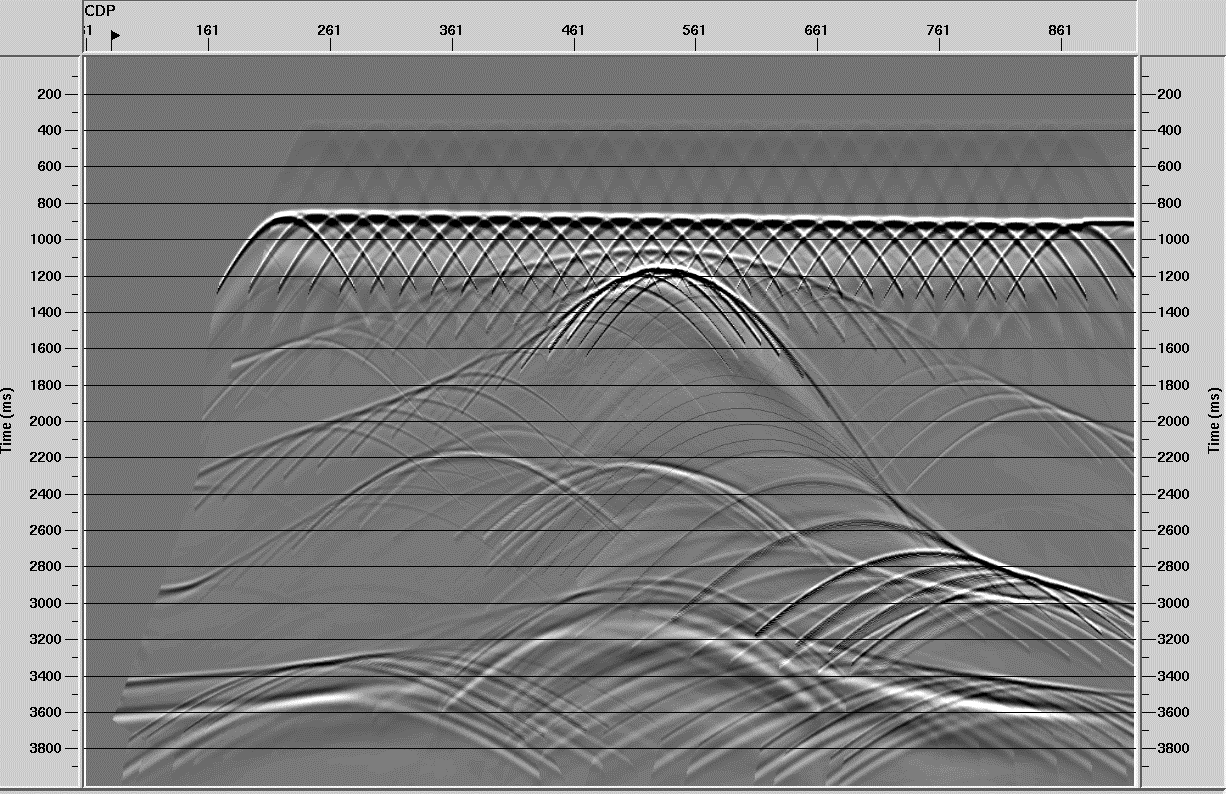
\includegraphics[scale=0.30]{images/simula_diff.png}
\vspace{-0.3cm}
\end{center}
\begin{center}
 Fonte: \cite{diffractions}.
\end{center}
\label{fig:8.1}
\end{figure}

\begin{figure}[htb]
\caption{Passo intermediário na determinação da velocidade de migração em loop.}
\begin{center}
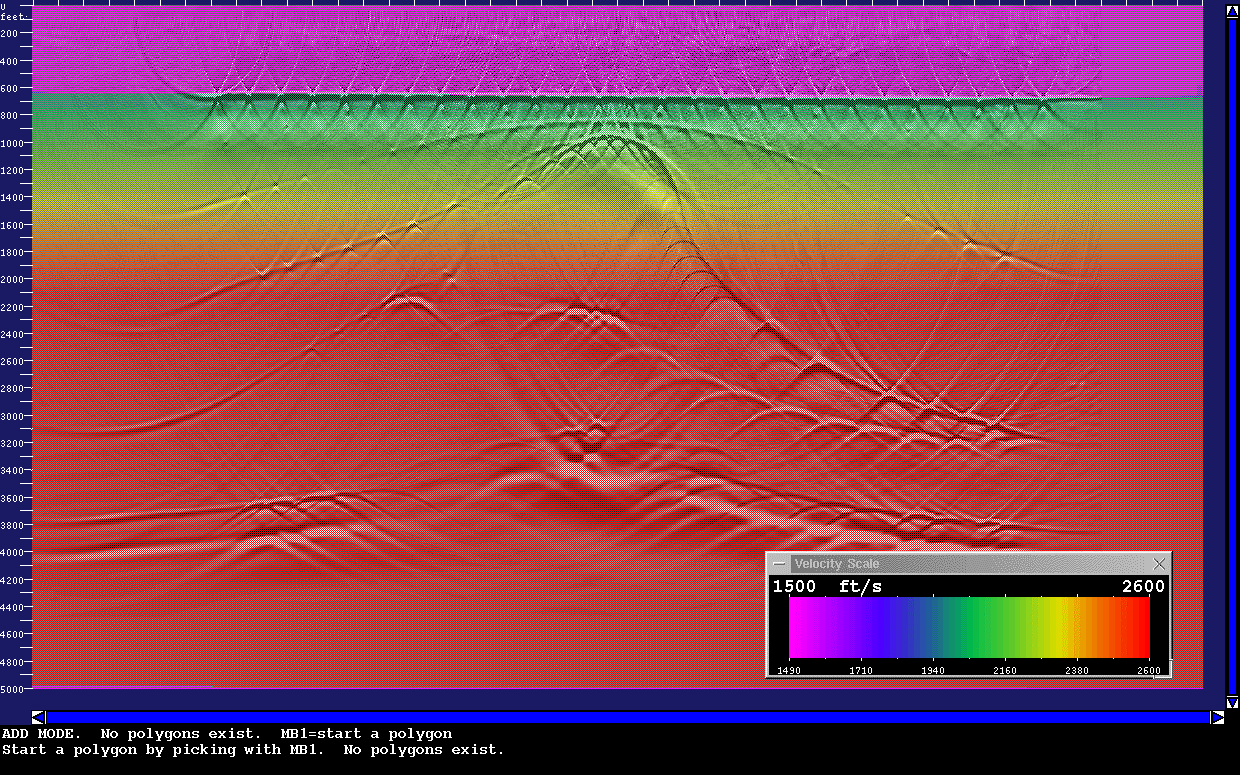
\includegraphics[scale=0.30]{images/simula_diff_campo.png}
\vspace{-0.3cm}
\end{center}
\begin{center}
 Fonte: \cite{diffractions}.
\end{center}
\label{fig:8.2}
\end{figure}

\begin{figure}[htb]
\caption{Imagem em profundidade obtido através da inversão a partir de respostas de difração simuladas 
em um modelo geológico sintético de uma estrutura salina.}
\begin{center}
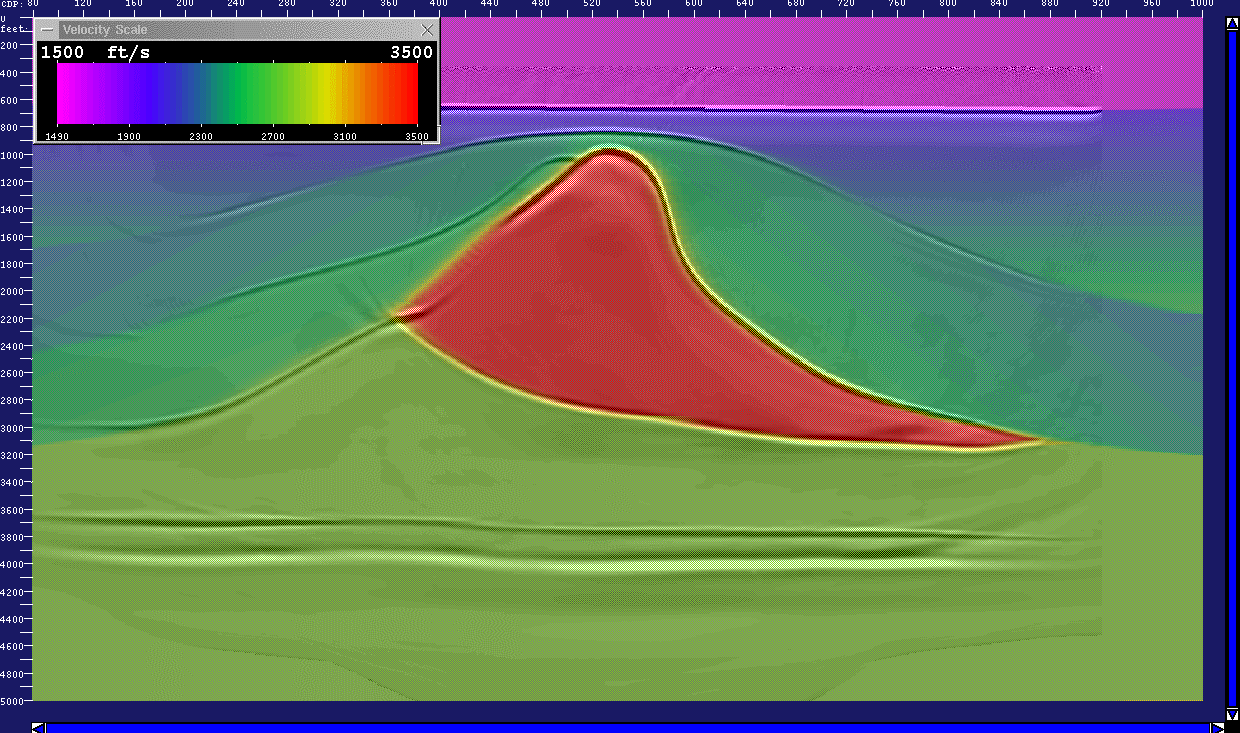
\includegraphics[scale=0.30]{images/simula_diff_vel.png}
\vspace{-0.3cm}
\end{center}
\begin{center}
 Fonte: \cite{diffractions}.
\end{center}
\label{fig:8.3}
\end{figure}

A análise de velocidades automatizada no domínio pós empilhado e o imageamento de alta resolução
para heterogeneidades de pequena escala serão feitos através da produção de seções migradas no tempo 
com as hipérboles de difração focalizadas. 
Este processo contará com a análise automatizada de focalização para a detecção das
velocidades de migração ótimas no imageamento das hipérboles de difração simuladas 
utilizando a medida de variação máxima local \cite{sep_dif}:

\begin{equation}
 \label{eq:8.2}
 \phi_i = \frac{\sum^N_{i=1} a_i }{\sqrt{ N \sum^N_{i=1} a_i^2 }} 
\end{equation}

Onde $s_i$ é a amplitude da amostra do sinal sísmico em uma janela de tamanho $N$.
Sinais bem focalizados possuem alta variação máxima local $\phi_i$. Desta forma, produziremos
os painéis de focalização de imagem calculando $\phi_i$ para cada ponto na seção migrada
e realizaremos a análise de velocidades automatizada (Um exemplo dos painéis de focalização de imagem
está na Figura \ref{fig:8.4}).

\begin{figure}[htb]
\caption{Exemplo de painéis de focalização de imagem. As cores representam os valores de variação
máxima local. O eixo das abcissas é a velocidade em Km/s. O eixo das ordenadas é o tempo em s.}
\begin{center}
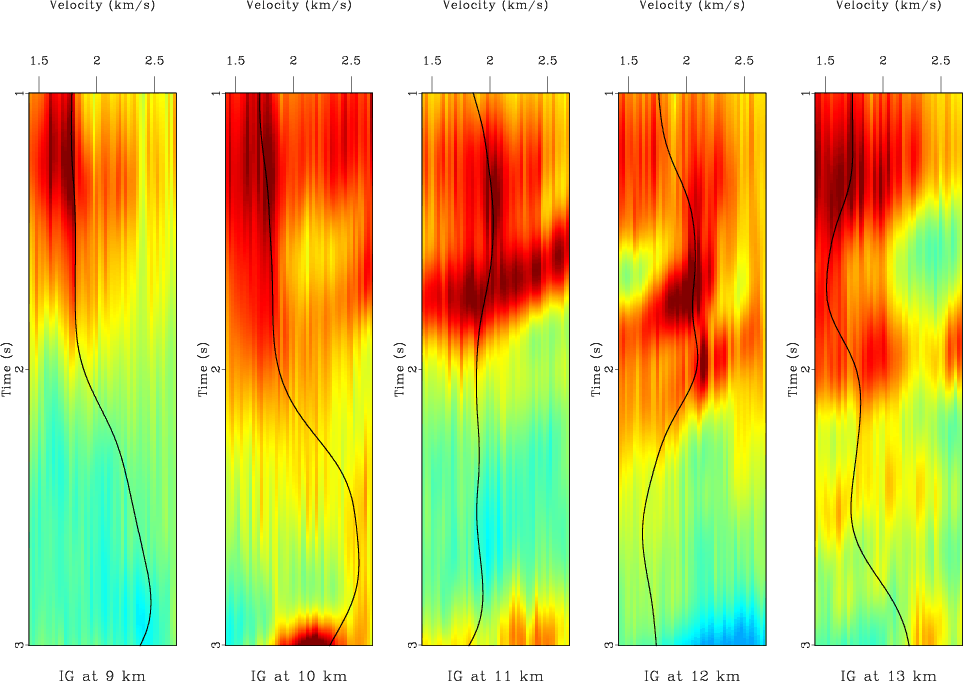
\includegraphics[scale=0.30]{images/panelfig.png}
\vspace{-0.3cm}
\end{center}
\begin{center}
 Fonte: \cite{sep_dif}.
\end{center}
\label{fig:8.4}
\end{figure}

A principal diferença desta metodologia para a análise
de velocidades convencional é que a informação sobre a velocidade
será obtida da focalização das difrações ao invés dos painéis de coerência \cite{sep_dif}.

A migração no tempo será realizada a partir de um algoritmo de continuação de velocidades \cite{fomel2003a},
um método que performa
a análise de velocidade de migração em tempo continuando imagens sísmicas na velocidade, também chamado de
``ondas imagem'' \cite{hubral1996}. A teoria da continuação de velocidades mostra ser possível realizar a migração no tempo
com um conjunto de diferentes velocidades fazendo pequenos incrementos na velocidade diretamente no domínio da imagem.
Implementaremos através de um algoritmo baseado na tranformada rápida de Fourier \cite{bfomel2003}.

A Figura \ref{fig:8.5} apresenta o algoritmo proposto para a obtenção do modelo de velocidades. O algoritmo funciona em um
laço seguindo os passos anteriormente descritos e a atualização do modelo de velocidades da iteração é realizada com
auxílio do VFSA até atingir um modelo ótimo. O critério de convergência será a coerência entre os dados modelados a partir do
o modelo de velocidades da iteração atual e os dados sísmicos pré empilhados \cite{mesquita}.

\begin{figure}[htb]
\caption{Fluxograma do algoritmo de inversão do modelo de velocidades.}
\begin{center}
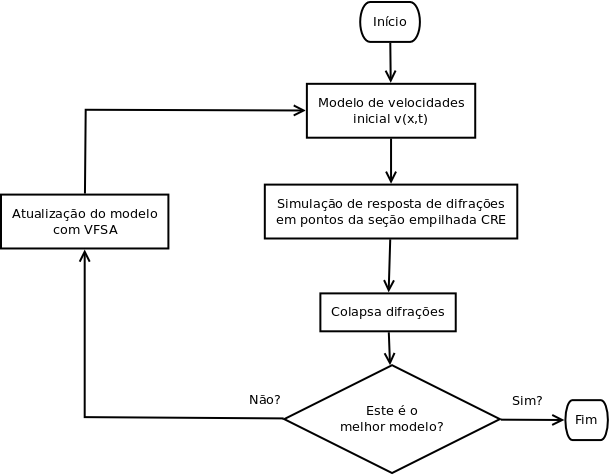
\includegraphics[scale=0.30]{images/fluxoVel.png}
\vspace{-0.3cm}
\end{center}
\begin{center}
 Fonte: Do Autor.
\end{center}
\label{fig:8.5}
\end{figure}